%%%%%%%%%%%%%%%%%%%% author.tex %%%%%%%%%%%%%%%%%%%%%%%%%%%%%%%%%%%
%
% sample root file for your "contribution" to a contributed volume
%
% Use this file as a template for your own input.
%
%%%%%%%%%%%%%%%% Springer %%%%%%%%%%%%%%%%%%%%%%%%%%%%%%%%%%%%%%%%%


% RECOMMENDED %%%%%%%%%%%%%%%%%%%%%%%%%%%%%%%%%%%%%%%%%%%%%%%%%%%
\documentclass[graybox]{svmult}

% choose options for [] as required from the list
% in the Reference Guide

\usepackage{mathptmx}       % selects Times Roman as basic font
\usepackage{helvet}         % selects Helvetica as sans-serif font
\usepackage{courier}        % selects Courier as typewriter font
\usepackage{type1cm}        % activate if the above 3 fonts are
                             % not available on your system

\usepackage{makeidx}         % allows index generation
\usepackage{graphicx}        % standard LaTeX graphics tool
                             % when including figure files
\usepackage{multicol}        % used for the two-column index
\usepackage[bottom]{footmisc}% places footnotes at page bottom

% TODO - can we get subcaption to work?  Else need to remove use of subfigures
\usepackage{subcaption}
\captionsetup{compatibility=false}
\usepackage{multirow}

\usepackage[
binary-units=true,
per-mode=symbol,
detect-weight=true,
]{siunitx}

% figure path and their extensions so you won't have to specify these with
% every instance of \includegraphics
\graphicspath{{figures/}}
\DeclareGraphicsExtensions{.pdf,.jpg,.png}


% TODO - biblio does not compile
\usepackage[
backend=biber,
%style=numeric, % Orders alphabetically by author last name
% style=ieee, % Orders by appearance in text
%citestyle=numeric-comp,
% citestyle=ieee,
%maxnames=6,
%minnames=1,
]{biblatex}

\bibliography{references}

% see the list of further useful packages
% in the Reference Guide

\makeindex             % used for the subject index
                       % please use the style svind.ist with
                       % your makeindex program

%%%%%%%%%%%%%%%%%%%%%%%%%%%%%%%%%%%%%%%%%%%%%%%%%%%%%%%%%%%%%%%%%%%%%%%%%%%%%%%%%%%%%%%%%

\begin{document}

\title{System Integration of RISC-V Processors with FD-SOI}
% Use \titlerunning{Short Title} for an abbreviated version of
% your contribution title if the original one is too long
\author{Ben Keller and Borivoje Nikoli\'{c}}
% Use \authorrunning{Short Title} for an abbreviated version of
% your contribution title if the original one is too long
\institute{Ben Keller \at NVIDIA Research, 2788 San Tomas Expressway, Santa Clara, CA 95051 \email{benk@nvidia.com}
\and Borivoje Nikoli\'{c} \at Department of Electrical Engineering and Computer Sciences, University of California, Berkeley, Berkeley, CA 94720 \email{bora@eecs.berkeley.edu}}
%
% Use the package "url.sty" to avoid
% problems with special characters
% used in your e-mail or web address
%
\maketitle

\abstract{TODO - abstract}

%-------------------------------------%
\section{SoC Design}

\subsection{Raven-3}

\subsection{Raven-4}


%-------------------------------------%
\section{RISC-V Processors}

\subsection{Rocket Chip}

The application core in Raven-3 implements the RV64G variant of the free and open RISC-V instruction set.
The processor, an instance of the Rocket Chip Generator~\cite{Rocket2016}, is a 64-bit five-stage single-issue in-order pipeline (see Figure~\ref{fig:6-raven3-rocket}).
The pipeline is carefully designed to minimize the impact of long clock-to-output delays of SRAM macros.
For example, the pipeline resolves branches in the memory stage to shorten the critical path through the bypass path, but relies on extensive branch prediction (a 64-entry branch target buffer, a 256-entry two-level branch history table, and a two-entry return address stack) to mitigate the increased branch resolution penalty.
The blocking \SI{16}{\kibi\byte} instruction cache is private to the Rocket core, while the nonblocking \SI{32}{\kibi\byte} data cache is shared between the scalar core and a vector coprocessor designed to accelerate data-parallel workloads.
The Rocket core has a memory-management unit that supports page-based virtual memory.
Both caches are virtually indexed and physically tagged, and have separate TLBs that are accessed in parallel with cache accesses.
The core has an IEEE 754-2008-compliant floating-point unit that executes single- and double-precision floating-point operations, including fused multiply-add (FMA) operations, with hardware support for subnormal numbers.

\begin{figure}
  \centering
  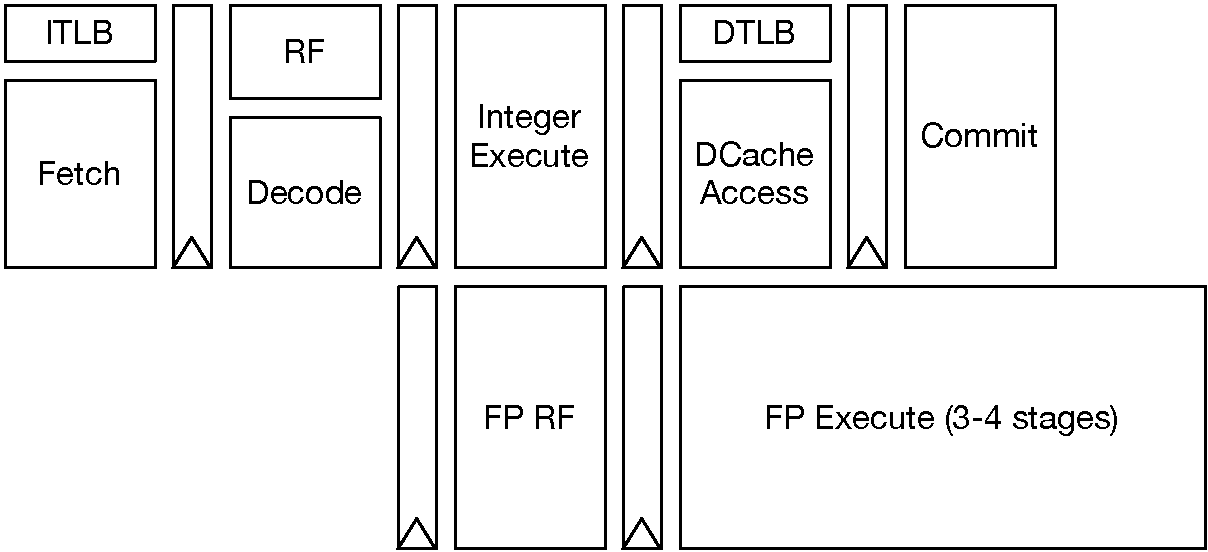
\includegraphics[width=0.8\textwidth]{6-raven3-rocket}
  \caption{A simplified pipeline diagram of the Rocket processor~\cite{Zimmer2016} ({\textcopyright} 2016 IEEE).}
  \label{fig:6-raven3-rocket}
\end{figure}

To reduce design complexity, the microprocessor is implemented as a tethered system.
Unlike a standalone system, a tethered system depends on a host machine to boot, and lacks I/O devices such as a console, mass storage, frame buffer, and network card.
The host (e.g., an x86 laptop) is connected to the target tethered system via the host-target interface (HTIF), a simple protocol that lets the host machine read and write target memory and control registers.
All I/O-related system calls are forwarded to the host machine using HTIF, where they are executed on behalf of the target.
Programs that run on the scalar core are downloaded into the target's memory via HTIF.
The resulting system is able to boot modern operating systems such as Linux utilizing I/O devices residing on the host machine, and can run standard applications such as the Python interpreter.


\subsection{Hwacha Vector Processor}

The Hwacha vector accelerator, shown in Figure~\ref{fig:6-raven3-hwacha}, is a decoupled single-lane vector unit tightly coupled with the Rocket core.
Hwacha executes vector operations temporally (split across subsequent cycles) rather than spatially (split across parallel datapaths), and has a vector length register that simplifies vector code generation and keeps the binary code compatible across different vector microarchitectures with different numbers of execution resources.
The Rocket scalar core sends vector memory instructions and vector fetch instructions to the vector accelerator.
A vector fetch instruction initiates execution of a block of vector arithmetic instructions.
The vector execution unit (VXU) fetches instructions from the private \SI{8}{\kibi\byte} vector instruction cache (VI\$), decodes instructions, clears hazards, and sequences vector instruction execution by sending multiple micro-ops down the vector lane.
The vector lane consists of a banked vector register file built out of two-ported SRAM macros, operand registers, per-bank integer ALUs, and long-latency functional units.
Multiple operands per cycle are read from the banked register file by exploiting the regular access pattern with operand registers used as temporary space~\cite{Lee2014}.
The long-latency functional units such as the integer multiplier and FMA units are shared between the Rocket core and the Hwacha accelerator.
The vector memory unit (VMU) supports unit-strided, constant-strided, and gather/scatter vector memory operations to the shared L1 data cache.
Vector memory instructions are also sent to the vector runahead unit (VRU) by the scalar core.
The VRU prefetches data blocks from memory and places them in the L1 data cache ahead of time to increase performance of vector memory operations executed by the VXU.
The resulting vector accelerator is more similar to traditional Cray-style vector pipelines~\cite{Russel1978} than SIMD units such as those that execute ARM's NEON or Intel's SSE/AVX instruction sets, and delivers high performance and energy efficiency while remaining area efficient.

\begin{figure}
  \centering
  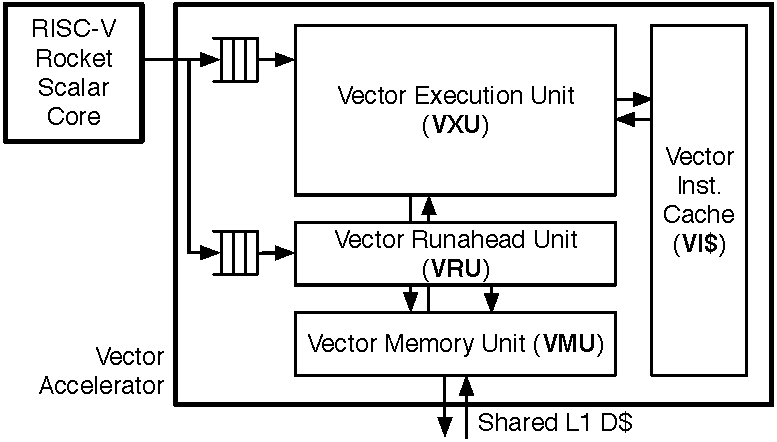
\includegraphics[width=0.65\textwidth]{6-raven3-hwacha}
  \caption{A block diagram of the Hwacha vector accelerator~\cite{Zimmer2016} ({\textcopyright} 2016 IEEE).}
  \label{fig:6-raven3-hwacha}
\end{figure}


%-------------------------------------%
\section{Energy-Efficient SRAMs}

Operation at low voltages is critical to achieving maximum energy efficiency, but on-chip SRAM typically limits the minimum operating voltage of the entire system as the small transistors in SRAM bitcells are especially vulnerable to process variation.
All SRAM arrays in the core voltage domain use the same custom 2KB 8T-based SRAM macro shown in Figure~\ref{fig:sram}, which is logically organized as 512 entries of 72 bits (64 bits + 8 possible ECC bits) and physically organized as two arrays of 128 rows by 144 columns with two-to-one physical interleaving.
Low-voltage operation is enabled by the 8T bitcell, where each transistor is larger than the equivalent high-density 6T bitcell, and by the FD-SOI process which reduces the threshold voltage variation \cite{planes}~\cite{raven1}.
While the arrays also implemented a negative bitline write assist, the assist was not necessary to achieve minimum voltage operation.

\begin{figure}
  \centering
  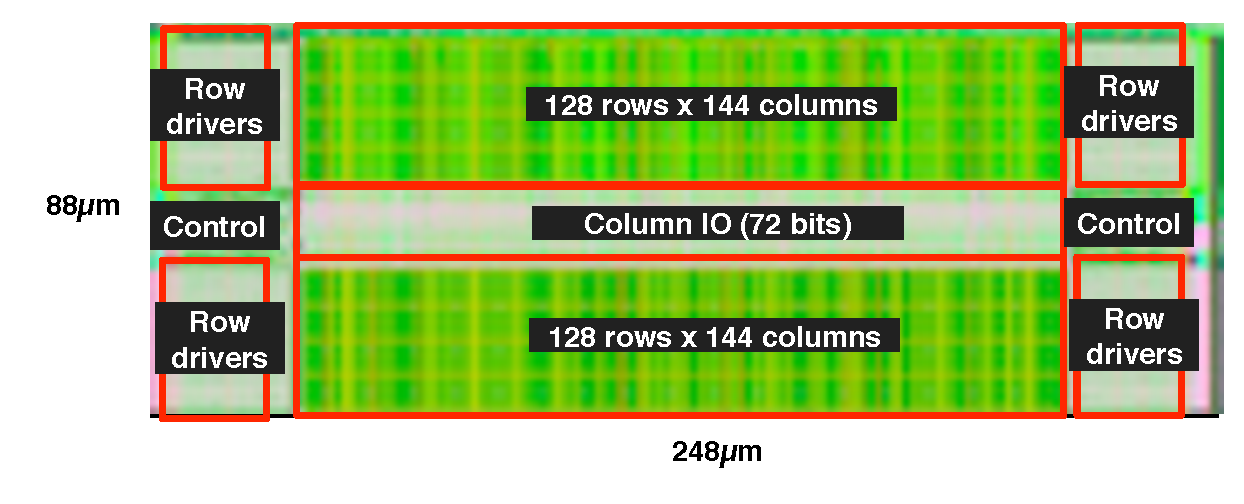
\includegraphics[width=0.7\textwidth]{sram}
  \caption{Layout of the custom 8T SRAM macro.}
  \label{fig:sram}
\end{figure}


%-------------------------------------%
\section{DC-DC Converters}

%\section{Simultaneous-Switching Switched-Capacitor Voltage Regulation}

Switched-capacitor voltage regulators are a favorable choice for integrated voltage regulation because high-quality integrated capacitors are much easier to implement than inductors, while switching regulator efficiencies exceed those of linear regulators.
However, as described in Section~\ref{sec:2-switch-cap}, switched-capacitor regulators typically achieve conversion efficiencies that are not high enough to justify their overhead. 
Energy savings from AVS are reduced by conversion losses to the extent that the additional area and design complexity required for their implementation were not worthwhile.
Accordingly, designing a switched-capacitor regulator with reasonably high efficiency is a critical component of a realistic FG-AVS system.

%\subsection{Traditional Switched-Capacitor Regulation}

Because each switching event in a switched-capacitor circuit is perturbing its output voltage with a discontinuous addition of charge, the output of switched-capacitor regulators tends to ripple.
Traditional switched-capacitor designs employ a technique known as interleaving to suppress this voltage ripple and produce a relatively flat output supply that is well-suited for synchronous digital logic \cite{Clerc2015, Jain2014, Jiang2017, Kim2015, Song2015, Teh2016}.
By dividing the total flying capacitance in the system into many smaller unit cells, and switching each of these unit cells out of phase with the others, the relative amount of charge delivered onto the supply with each switching event is small, and the output voltage ripple is minimized as shown in Figure~\ref{fig:3-simultaneous-switching-a}.
High interleaving phase counts of 16, 32, or even greater can be used to suppress the ripple and produce a steady output voltage \cite{Andersen2014, Le2011, Pique2012}.
However, this interleaved approach suffers from charge-sharing losses as each unit cell shares charge across the flying capacitance of the others when it switches.
These intrinsic charge-sharing losses comprise up to 40\% of the overall energy losses in the voltage conversion~\cite{Jevtic2014}.

\begin{figure}
  \centering
  \hspace*{\fill}
  \begin{subfigure}[t]{0.42\textwidth}
  \centering
  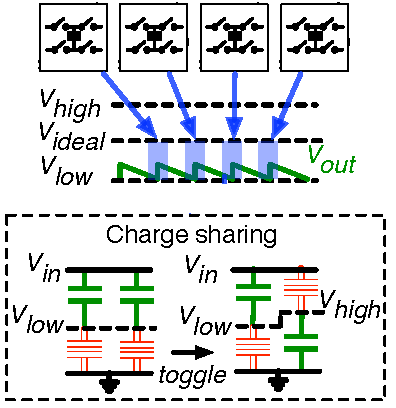
\includegraphics[width=\textwidth]{3-simultaneous-switching-a}
  \caption{}
  \label{fig:3-simultaneous-switching-a}
  \end{subfigure}
  \hspace*{\fill}
  \begin{subfigure}[t]{0.42\textwidth}
  \centering
  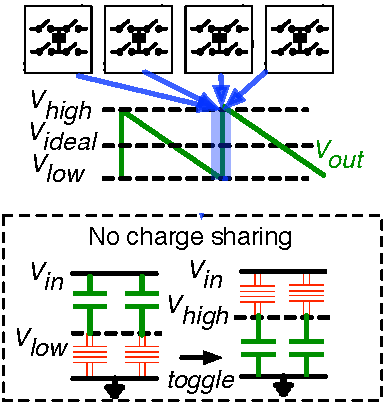
\includegraphics[width=\textwidth]{3-simultaneous-switching-b}
  \caption{}
  \label{fig:3-simultaneous-switching-b}
  \end{subfigure}
  \hspace*{\fill}
  \caption{Interleaved and simultaneous-switching switched-capacitor DC-DC converters~\cite{Zimmer2016}.  In the four-phase interleaved converter shown in (\subref{fig:3-simultaneous-switching-a}), each unit cell switches out of phase with the others, resulting in a relatively flat output voltage but incurring charge-sharing losses.  In the simultaneous-switching converter shown in (\subref{fig:3-simultaneous-switching-b}), all unit cells switch at once, eliminating charge-sharing losses but resulting in a large output voltage ripple.}
  \label{fig:3-simultaneous-switching}
\end{figure}

The conversion losses of switched-capacitor voltage regulators are composed of four parts, three of which depend on the switching frequency of the design~\cite{Le2011}.
The intrinsic charge-sharing loss $P_{cfly}$ of switched-capacitor designs is inversely proportional to the switching frequency of the design, because a slower switching frequency means more charge being transferred for each switching event.
The bottom-plate conduction loss $P_{bottom}$ caused by the parasitic capacitance of the flying capacitor to ground and the parasitic gate capacitance $P_{gate}$ of the switches are both directly proportional to the switching frequency.
The conduction loss $P_{cond}$ through the switches does not depend on switching frequency.
Switched-capacitor designs typically operate at the optimal switching frequency to minimize the total losses in the system, operating fast enough to reduce charge-sharing losses but not so fast that the parasitic losses dominate.

%\subsection{Simultaneous-Switching Switched-Capacitor Regulation}
%\label{sec:3-sc-dcdc}

An alternative approach called simultaneous switching is shown in Figure~\ref{fig:3-simultaneous-switching-b}.
Instead of interleaving the unit cells, the entire flying capacitance of the regulator is switched at once, eliminating all charge-sharing between different unit cells present in the interleaved approach~\cite{Zimmer2016}.
The elimination of this loss term also means that the only losses remaining in the system are either directly proportional to switching frequency or agnostic to it, so the switching frequency of the system can be reduced, further shrinking remaining losses.
Figure~\ref{fig:3-dcdc-analysis} shows analytical results comparing the losses from an interleaved system with those of a simultaneous-switching regulator driving an ideal resistive load.
The simultaneous-switching switched-capacitor DC-DC (SS-SC) converter is able to achieve total losses of less than 10\% by slowing its switching frequency.
In real systems, the load is not purely resistive, but instead has some capacitive component, so charge-sharing losses are not eliminated entirely.
Figure~\ref{fig:3-dcdc-analysis-cap} shows a simulated example of how the inclusion of a capacitive load in the SS-SC circuit diminishes some of the advantage of the simultaneous-switching design and increases the most efficient switching frequency relative to a purely resistive load.
Nonetheless, the energy savings over the interleaved approach remain substantial, and the optimal switching frequency is lower in the SS-SC design.

\begin{figure}
  \centering
  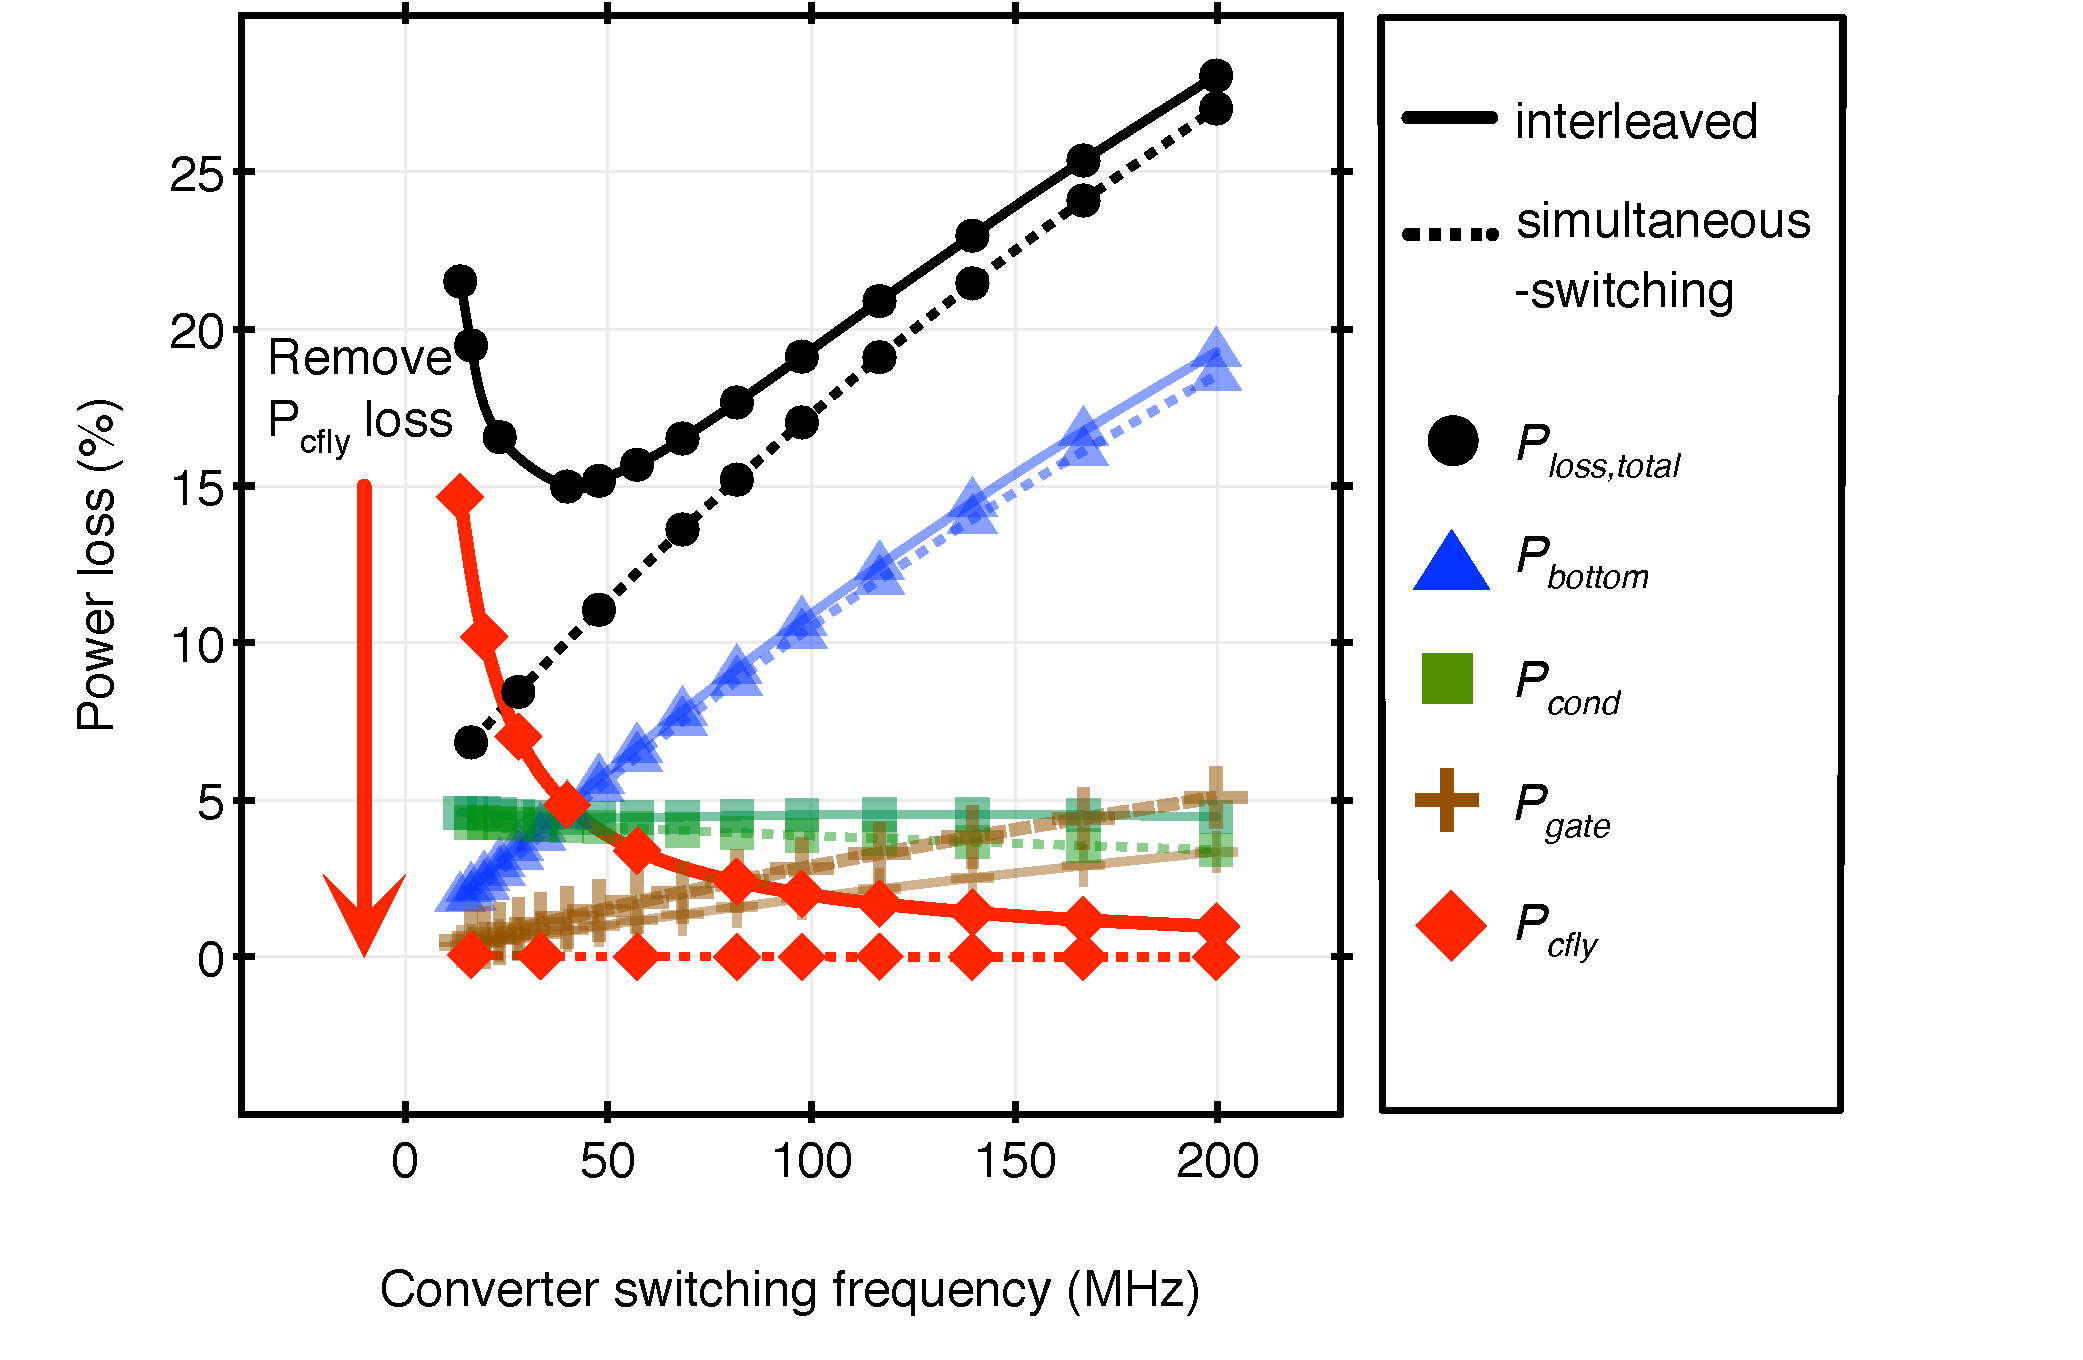
\includegraphics[width=0.8\textwidth]{3-dcdc-analysis}
  \caption{Analytical results showing the efficiency improvement of the simultaneous-switching switched-capacitor voltage regulator~\cite{Zimmer2016} ({\textcopyright} 2016 IEEE).}
  \label{fig:3-dcdc-analysis}
\end{figure}

\begin{figure}
  \centering
  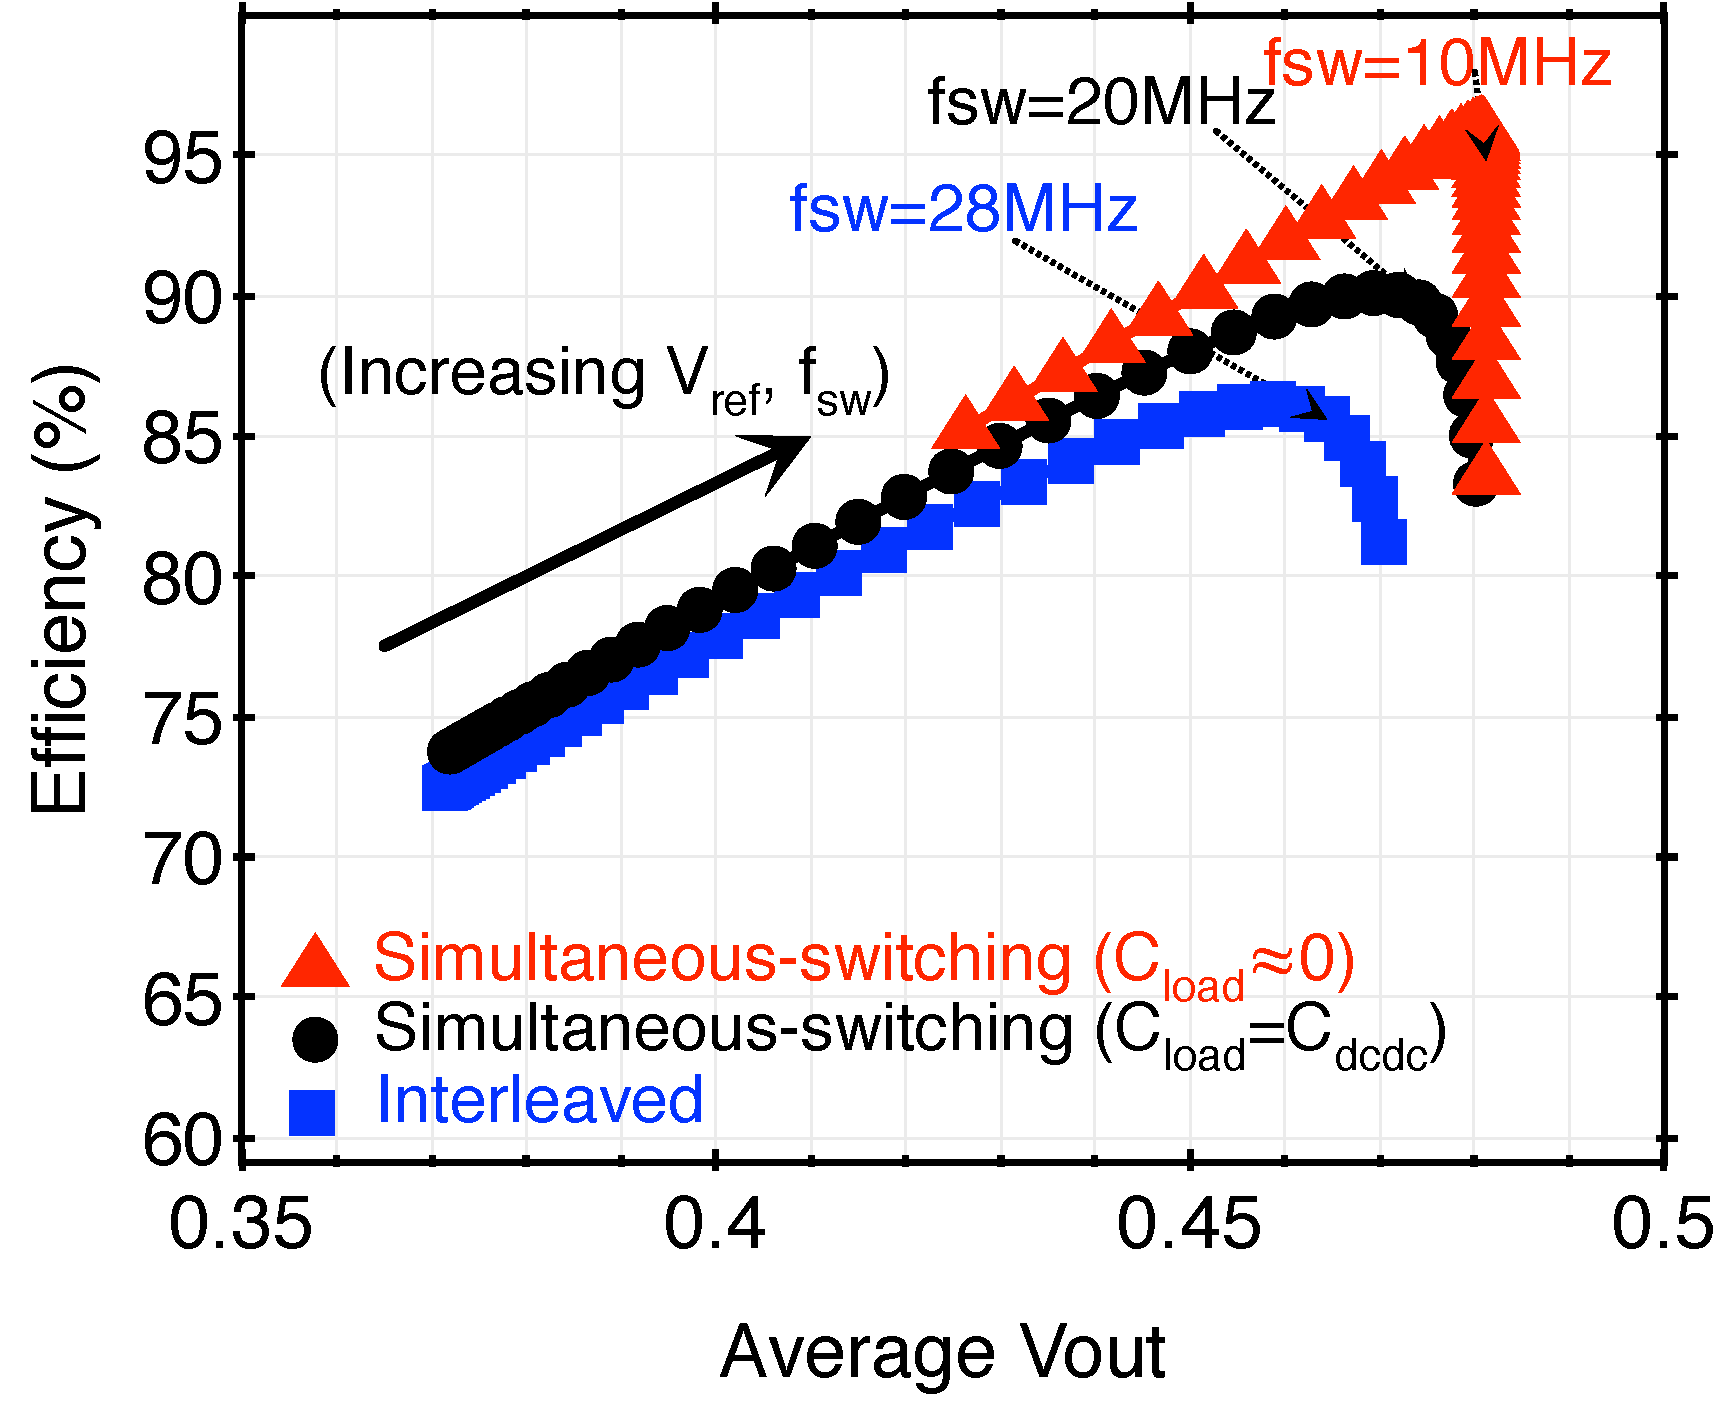
\includegraphics[width=0.6\textwidth]{3-dcdc-analysis-cap}
  \caption{Simulation results showing the impact of load capacitance on converter efficiency and switching frequency~\cite{Zimmer2016} ({\textcopyright} 2016 IEEE).}
  \label{fig:3-dcdc-analysis-cap}
\end{figure}

Simultaneous-switching designs reduce the loss components associated with switched-capacitor regulation, but they generate an output voltage that ripples substantially around an average.
This rippling supply is not well-suited to a traditional synchronous digital system operating at a fixed clock frequency, because the digital clock must operate at a slower frequency corresponding to the lowest voltage of the ripple in order to guarantee safe operation.
This would result in wasted energy as the rippling voltage exceeds its minimum, as shown in Figure~\ref{fig:3-ripple-clocking-a}, and these over-voltage losses would exceed the savings from the elimination of charge sharing.
Systems employing SS-SC regulators therefore require the clock supplied to the digital load to adapt to the changing voltage in order to achieve reasonable efficiencies~\cite{Jevtic2014}.
As shown in Figure~\ref{fig:3-ripple-clocking-b}, by changing the clock on a cycle-by-cycle basis to match the instantaneous operating conditions of the load, the over-voltage losses can be eliminated.

\begin{figure}
  \centering
%  \hspace*{\fill}
  \begin{subfigure}[t]{0.6\textwidth}
  \centering
  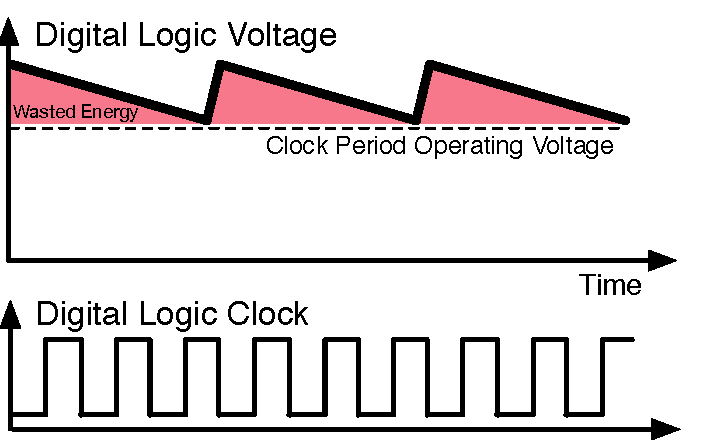
\includegraphics[width=\textwidth]{3-ripple-clocking-a}
  \caption{}
  \label{fig:3-ripple-clocking-a}
  \end{subfigure}
%  \hspace*{\fill}
  \par\bigskip
  \begin{subfigure}[t]{0.6\textwidth}
  \centering
  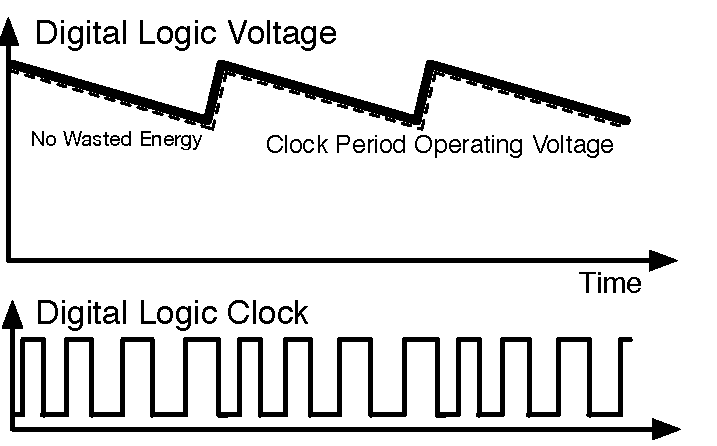
\includegraphics[width=\textwidth]{3-ripple-clocking-b}
  \caption{}
  \label{fig:3-ripple-clocking-b}
  \end{subfigure}
%  \hspace*{\fill}
  \caption{Sample voltage and clock waveforms of SS-SC systems.  In (\subref{fig:3-ripple-clocking-a}), the clock does not adapt to the voltage ripple, so it must be margined for the lowest supply voltage, resulting in wasted energy at higher voltages.  In (\subref{fig:3-ripple-clocking-b}), the clock adapts to the voltage ripple, allowing the circuit to speed up when the voltage is higher than the minimum.}
  \label{fig:3-ripple-clocking}
\end{figure}
 
%\subsection{Regulator Design}

Traditional switched-capacitor regulators achieve peak efficiencies when supplying output voltages at discrete levels determined by their topology.
While SS-SC regulators do not generate a fixed output voltage, their efficiency still peaks at a particular average output level.
As a wide range of voltages are desirable for FG-AVS, a reconfigurable switching network with a topology similar to that of \cite{Le2011} was implemented.
The design can operate in four different modes that generate voltages from fixed \SI{1}{\volt} and \SI{1.8}{\volt} supplies.
The \SI{1.8}{\volt} 1/2 mode downconverts the \SI{1.8}{\volt} input in a 2:1 ratio, resulting in an average output voltage around \SI{900}{\milli\volt}.
The \SI{1}{\volt} 2/3 mode and \SI{1}{\volt} 1/2 mode each downconvert the 1.0V input, resulting in average output voltages of roughly \SI{667}{\milli\volt} and \SI{500}{\milli\volt} respectively.
A bypass mode connects the \SI{1}{\volt} input directly to the output rail.
The design re-uses the flying capacitance and switches, reconfiguring the switching pattern between each topology to avoid area overhead (see Figure~\ref{fig:3-dcdc-topologies}).

\begin{figure}
  \centering
  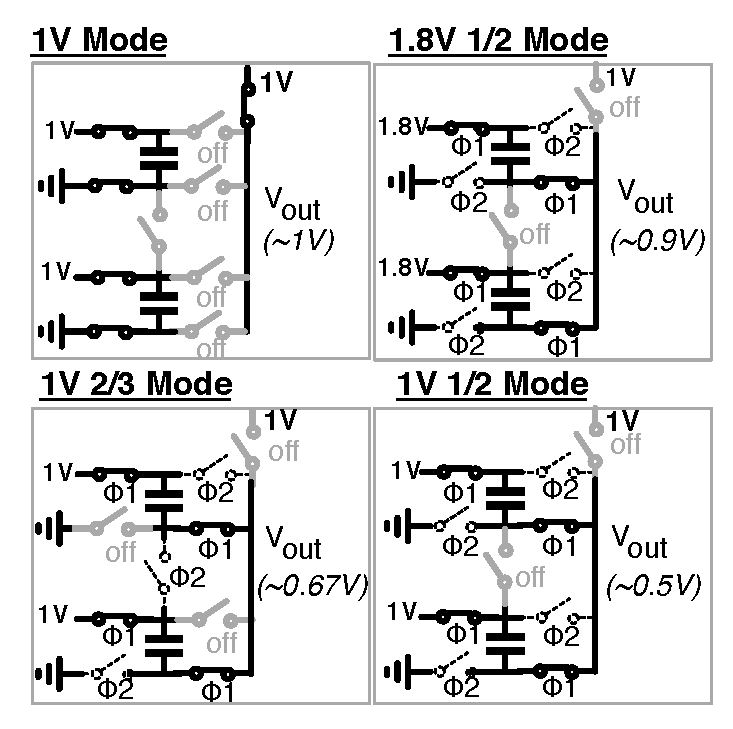
\includegraphics[width=0.6\textwidth]{3-dcdc-topologies}
  \caption{The four topologies of the reconfigurable SS-SC converter~\cite{Zimmer2016} ({\textcopyright} 2016 IEEE).}
  \label{fig:3-dcdc-topologies}
\end{figure}

The phases and configurations of the switches in the SS-SC regulator are set by a finite-state-machine controller.
This logic is responsible for configuring and reconfiguring the topology of the regulator, as well as switching between the two operating phases to pump charge onto the output of the converter.
The regulator topology is determined by setting a control register that, when changed, triggers a reconfiguration between voltage modes.
To generate the toggle clock that is distributed to the switches in the regulator, a comparator circuit acting on a \SI{2}{\GHz} clock detects when the regulated output voltage drops below a fixed external reference.
When the comparator triggers, control logic produces the next toggle clock edge, switching the SS-SC toggle clock phase and causing more charge to be supplied, boosting the voltage.
As a different reference voltage is needed for each mode, different comparators must be implemented to function in the appropriate voltage ranges (see Figure~\ref{fig:3-dcdc-comparators}).
In the event that one switching event does not sufficiently increase the generated voltage to bring it above the reference voltage, additional logic triggers further switching events after a delay, ensuring that the voltage will eventually be boosted back up to nominal levels.
The state machine controller is diagrammed in Figure~\ref{fig:3-dcdc-state-machine}.

\begin{figure}
  \centering
  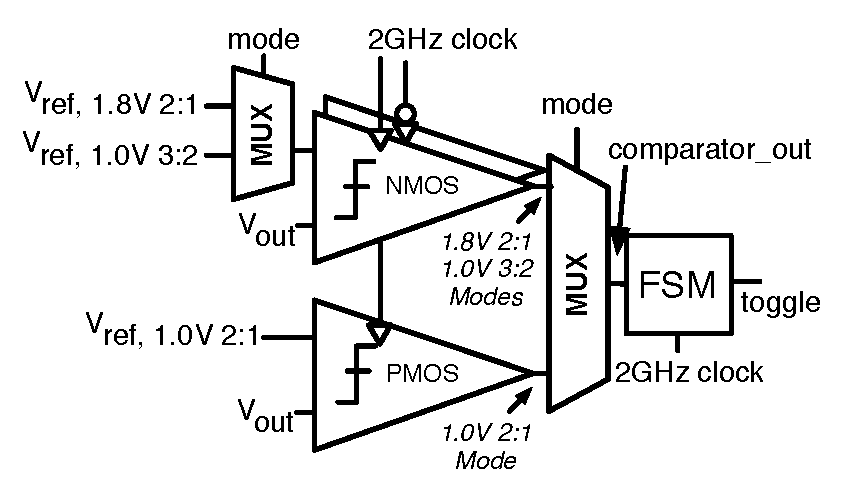
\includegraphics[width=0.6\textwidth]{3-dcdc-comparators}
  \caption{A diagram of the comparators used in the SS-SC controller~\cite{Zimmer2016} ({\textcopyright} 2016 IEEE).  Different comparators are needed to accommodate the voltage ranges of the references for the three different switching modes.}
  \label{fig:3-dcdc-comparators}
\end{figure}

\begin{figure}
  \centering
  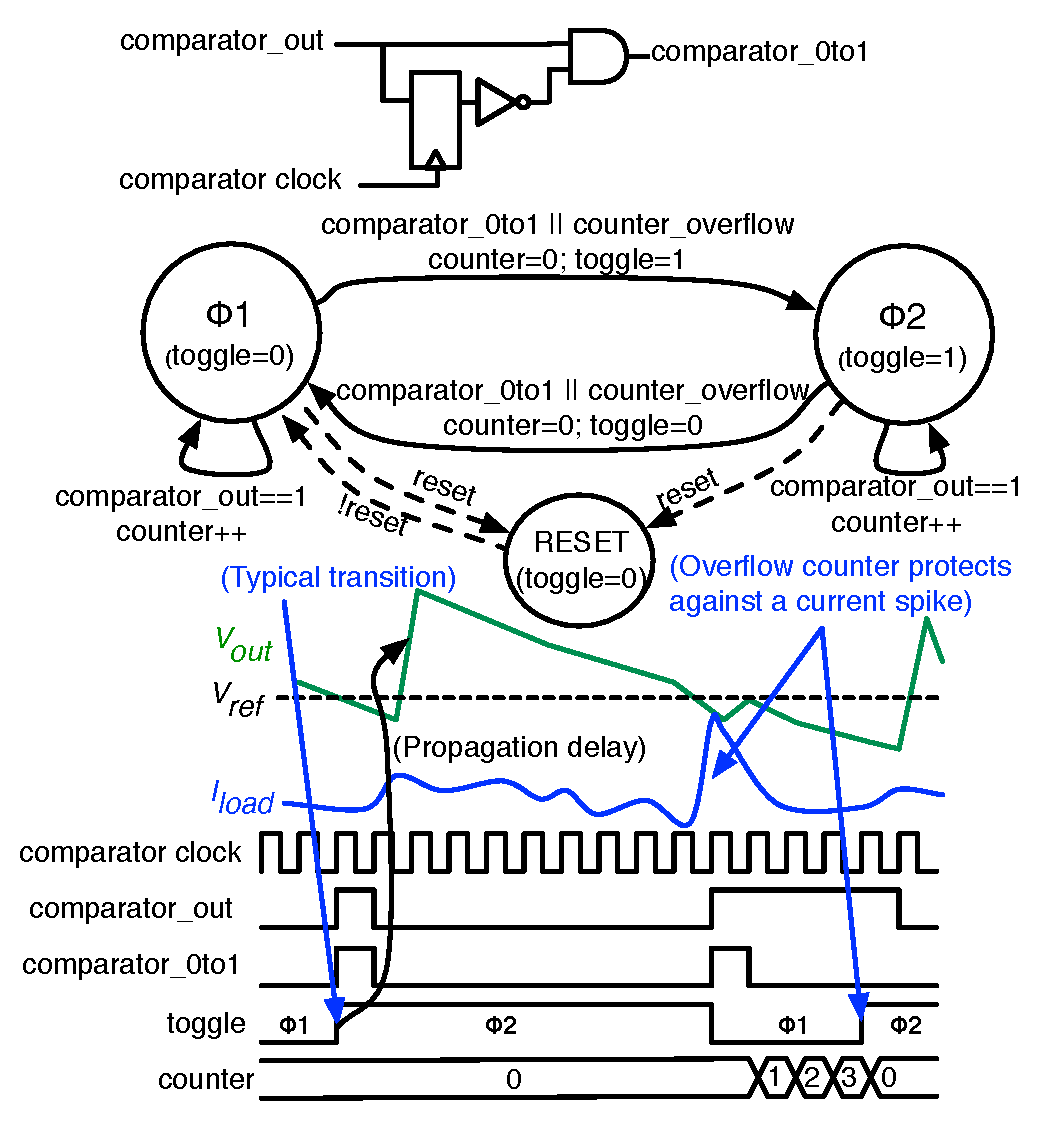
\includegraphics[width=0.8\textwidth]{3-dcdc-state-machine}
  \caption{The state machine used in the SS-SC controller and example waveforms of its operation~\cite{Zimmer2016} ({\textcopyright} 2016 IEEE).  If the current demand increases as the converter is toggling, the voltage may not rise about $V_{ref}$, so an additional counter triggers further switching until the voltage increases.}
  \label{fig:3-dcdc-state-machine}
\end{figure}

%-------------------------------------%
\section{Body-Bias Generation}
Pull from Miki's VLSI paper.

\section{Clock Generation}

Section~\ref{sec:2-clocking} described the utility of distributed, localized clock generation in the implementation of the GALS design style required for FG-AVS systems.
Furthermore, because SS-SC converters generate a rippling supply voltage, only a clock that adjusts to this ripple on a cycle-by-cycle basis to supply the digital logic can avoid wasted energy in these systems.
Accordingly, a local adaptive clock generator was implemented that can be paired with the SS-SC converter for FG-AVS systems~\cite{Keller2017}.

A block diagram of the clock generator circuit is shown in Figure~\ref{fig:3-clockgen}.
The adaptive clock generator is free-running and does not require any external reference.
The circuit generates clock edges via a D flip-flop, which is set or reset with pulse generators to toggle between one and zero.
After a rising clock edge is generated, the edge propagates through the first delay unit and then triggers a reset pulse on the flip-flop, causing the output to fall.
This edge then continues through the second delay unit and triggers a clock pulse on the flip-flop, resulting in a rising edge at the output.
This design allows the duty cycle of the generated clock to be adjusted.

\begin{figure}
  \centering
  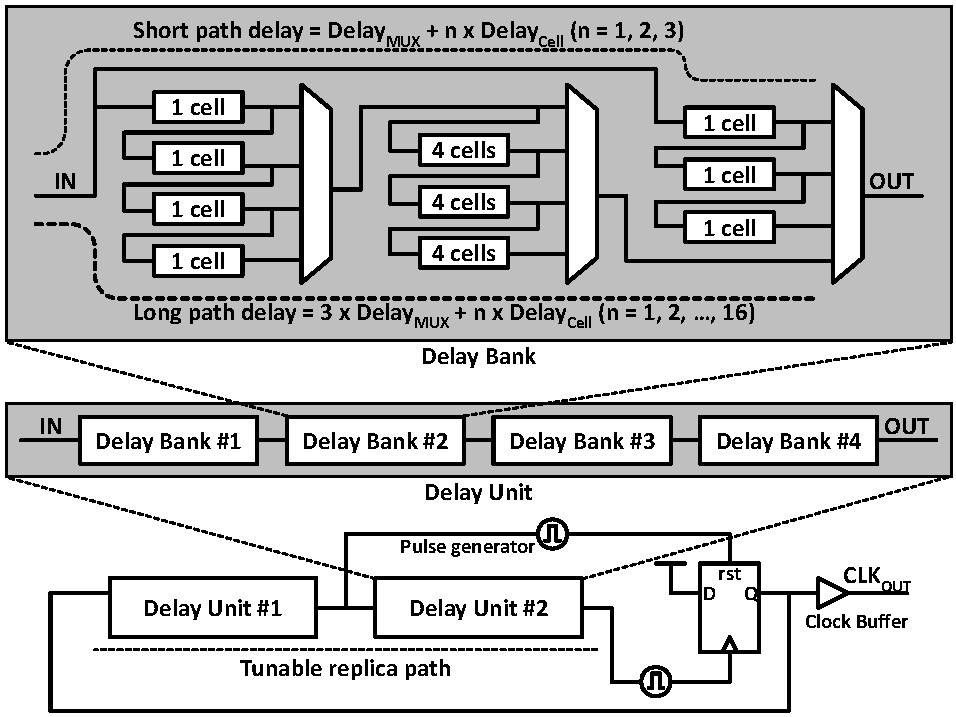
\includegraphics[width=0.8\textwidth]{3-clockgen}
  \caption{A block diagram of the adaptive clock generator~\cite{Keller2017} ({\textcopyright} 2017 IEEE).}
  \label{fig:3-clockgen}
\end{figure}

The adaptive clock generator is supplied by the same rippling output voltage that is used to power the digital logic in the system.
The delay units therefore respond to voltage changes similarly to the digital logic; the propagation delays that trigger each clock edge face the same environment as the digital logic paths in the design.
Each delay unit is comprised of four delay banks, and each bank consists of a chain of a particular cell in addition to multiplexors and control logic that allow the number of cells in the delay chain to be selected.
The first bank uses a custom buffer cell design to balance rise and fall times.
Each of the remaining banks consists of a standard cell that was commonly observed in the synthesized critical paths of the digital logic.
Each bank uses a different combination of pMOS/nMOS ratio and gate length, as these characteristics affect the voltage-frequency relationship of the cells.
By selecting different mux settings, the delay paths can be tuned until they match the delay characteristics of the critical paths in the digital logic supplied by the generated clock, ensuring that the clock edges are generated at the appropriate frequency for the instantaneous voltage produced by the regulator.

\section{System Performance}

\begin{acknowledgement}
TODO - acknowledgement
\end{acknowledgement}

%%%%%%%%%%%%%%%%%%%%%%%% referenc.tex %%%%%%%%%%%%%%%%%%%%%
% sample references
% 
% Use this file as a template for your own input.
%
%%%%%%%%%%%%%%%%%%%%%%%% Springer%%%%%%%%%%%%%%%%%%%%%%%%%%
%
% BibTeX users please use
% \bibliographystyle{}
% \bibliography{}
%
\biblstarthook{References may be \textit{cited} in the text either by number (preferred) or by author/year.\footnote{Make sure that all references from the list are cited in the text. Those not cited should be moved to a separate \textit{Further Reading} section or chapter.} The reference list should ideally be \textit{sorted} in alphabetical order -- even if reference numbers are used for the their citation in the text. If there are several works by the same author, the following order should be used: 
\begin{enumerate}
\item all works by the author alone, ordered chronologically by year of publication
\item all works by the author with a coauthor, ordered alphabetically by coauthor
\item all works by the author with several coauthors, ordered chronologically by year of publication.
\end{enumerate}
The \textit{styling} of references\footnote{Always use the standard abbreviation of a journal's name according to the ISSN \textit{List of Title Word Abbreviations}, see \url{http://www.issn.org/en/node/344}} depends on the subject of your book:
\begin{itemize}
\item The \textit{two} recommended styles for references in books on \textit{mathematical, physical, statistical and computer sciences} are depicted in ~\cite{science-contrib, science-online, science-mono, science-journal, science-DOI} and ~\cite{phys-online, phys-mono, phys-journal, phys-DOI, phys-contrib}.
\item Examples of the most commonly used reference style in books on \textit{Psychology, Social Sciences} are~\cite{psysoc-mono, psysoc-online,psysoc-journal, psysoc-contrib, psysoc-DOI}.
\item Examples for references in books on \textit{Humanities, Linguistics, Philosophy} are~\cite{humlinphil-journal, humlinphil-contrib, humlinphil-mono, humlinphil-online, humlinphil-DOI}.
\item Examples of the basic Springer style used in publications on a wide range of subjects such as \textit{Computer Science, Economics, Engineering, Geosciences, Life Sciences, Medicine, Biomedicine} are ~\cite{basic-contrib, basic-online, basic-journal, basic-DOI, basic-mono}. 
\end{itemize}
}

\begin{thebibliography}{99.}%
% and use \bibitem to create references.
%
% Use the following syntax and markup for your references if 
% the subject of your book is from the field 
% "Mathematics, Physics, Statistics, Computer Science"
%
% Contribution 
\bibitem{science-contrib} Broy, M.: Software engineering --- from auxiliary to key technologies. In: Broy, M., Dener, E. (eds.) Software Pioneers, pp. 10-13. Springer, Heidelberg (2002)
%
% Online Document
\bibitem{science-online} Dod, J.: Effective substances. In: The Dictionary of Substances and Their Effects. Royal Society of Chemistry (1999) Available via DIALOG. \\
\url{http://www.rsc.org/dose/title of subordinate document. Cited 15 Jan 1999}
%
% Monograph
\bibitem{science-mono} Geddes, K.O., Czapor, S.R., Labahn, G.: Algorithms for Computer Algebra. Kluwer, Boston (1992) 
%
% Journal article
\bibitem{science-journal} Hamburger, C.: Quasimonotonicity, regularity and duality for nonlinear systems of partial differential equations. Ann. Mat. Pura. Appl. \textbf{169}, 321--354 (1995)
%
% Journal article by DOI
\bibitem{science-DOI} Slifka, M.K., Whitton, J.L.: Clinical implications of dysregulated cytokine production. J. Mol. Med. (2000) doi: 10.1007/s001090000086 
%
\bigskip

% Use the following (APS) syntax and markup for your references if 
% the subject of your book is from the field 
% "Mathematics, Physics, Statistics, Computer Science"
%
% Online Document
\bibitem{phys-online} J. Dod, in \textit{The Dictionary of Substances and Their Effects}, Royal Society of Chemistry. (Available via DIALOG, 1999), 
\url{http://www.rsc.org/dose/title of subordinate document. Cited 15 Jan 1999}
%
% Monograph
\bibitem{phys-mono} H. Ibach, H. L\"uth, \textit{Solid-State Physics}, 2nd edn. (Springer, New York, 1996), pp. 45-56 
%
% Journal article
\bibitem{phys-journal} S. Preuss, A. Demchuk Jr., M. Stuke, Appl. Phys. A \textbf{61}
%
% Journal article by DOI
\bibitem{phys-DOI} M.K. Slifka, J.L. Whitton, J. Mol. Med., doi: 10.1007/s001090000086
%
% Contribution 
\bibitem{phys-contrib} S.E. Smith, in \textit{Neuromuscular Junction}, ed. by E. Zaimis. Handbook of Experimental Pharmacology, vol 42 (Springer, Heidelberg, 1976), p. 593
%
\bigskip
%
% Use the following syntax and markup for your references if 
% the subject of your book is from the field 
% "Psychology, Social Sciences"
%
%
% Monograph
\bibitem{psysoc-mono} Calfee, R.~C., \& Valencia, R.~R. (1991). \textit{APA guide to preparing manuscripts for journal publication.} Washington, DC: American Psychological Association.
%
% Online Document
\bibitem{psysoc-online} Dod, J. (1999). Effective substances. In: The dictionary of substances and their effects. Royal Society of Chemistry. Available via DIALOG. \\
\url{http://www.rsc.org/dose/Effective substances.} Cited 15 Jan 1999.
%
% Journal article
\bibitem{psysoc-journal} Harris, M., Karper, E., Stacks, G., Hoffman, D., DeNiro, R., Cruz, P., et al. (2001). Writing labs and the Hollywood connection. \textit{J Film} Writing, 44(3), 213--245.
%
% Contribution 
\bibitem{psysoc-contrib} O'Neil, J.~M., \& Egan, J. (1992). Men's and women's gender role journeys: Metaphor for healing, transition, and transformation. In B.~R. Wainrig (Ed.), \textit{Gender issues across the life cycle} (pp. 107--123). New York: Springer.
%
% Journal article by DOI
\bibitem{psysoc-DOI}Kreger, M., Brindis, C.D., Manuel, D.M., Sassoubre, L. (2007). Lessons learned in systems change initiatives: benchmarks and indicators. \textit{American Journal of Community Psychology}, doi: 10.1007/s10464-007-9108-14.
%
%
% Use the following syntax and markup for your references if 
% the subject of your book is from the field 
% "Humanities, Linguistics, Philosophy"
%
\bigskip
%
% Journal article
\bibitem{humlinphil-journal} Alber John, Daniel C. O'Connell, and Sabine Kowal. 2002. Personal perspective in TV interviews. \textit{Pragmatics} 12:257--271
%
% Contribution 
\bibitem{humlinphil-contrib} Cameron, Deborah. 1997. Theoretical debates in feminist linguistics: Questions of sex and gender. In \textit{Gender and discourse}, ed. Ruth Wodak, 99--119. London: Sage Publications.
%
% Monograph
\bibitem{humlinphil-mono} Cameron, Deborah. 1985. \textit{Feminism and linguistic theory.} New York: St. Martin's Press.
%
% Online Document
\bibitem{humlinphil-online} Dod, Jake. 1999. Effective substances. In: The dictionary of substances and their effects. Royal Society of Chemistry. Available via DIALOG. \\
http://www.rsc.org/dose/title of subordinate document. Cited 15 Jan 1999
%
% Journal article by DOI
\bibitem{humlinphil-DOI} Suleiman, Camelia, Daniel C. O�Connell, and Sabine Kowal. 2002. `If you and I, if we, in this later day, lose that sacred fire...�': Perspective in political interviews. \textit{Journal of Psycholinguistic Research}. doi: 10.1023/A:1015592129296.
%
%
%
\bigskip
%
%
% Use the following syntax and markup for your references if 
% the subject of your book is from the field 
% "Computer Science, Economics, Engineering, Geosciences, Life Sciences"
%
%
% Contribution 
\bibitem{basic-contrib} Brown B, Aaron M (2001) The politics of nature. In: Smith J (ed) The rise of modern genomics, 3rd edn. Wiley, New York 
%
% Online Document
\bibitem{basic-online} Dod J (1999) Effective Substances. In: The dictionary of substances and their effects. Royal Society of Chemistry. Available via DIALOG. \\
\url{http://www.rsc.org/dose/title of subordinate document. Cited 15 Jan 1999}
%
% Journal article by DOI
\bibitem{basic-DOI} Slifka MK, Whitton JL (2000) Clinical implications of dysregulated cytokine production. J Mol Med, doi: 10.1007/s001090000086
%
% Journal article
\bibitem{basic-journal} Smith J, Jones M Jr, Houghton L et al (1999) Future of health insurance. N Engl J Med 965:325--329
%
% Monograph
\bibitem{basic-mono} South J, Blass B (2001) The future of modern genomics. Blackwell, London 
%
\end{thebibliography}


\printbibliography

\end{document}





% Original Springer template is below


%\section{Section Heading}
%\label{sec:1}
%Use the template \emph{chapter.tex} together with the Springer document class SVMono (monograph-type books) or SVMult (edited books) to style the various elements of your chapter content in the Springer layout.
%
%Instead of simply listing headings of different levels we recommend to let every heading be followed by at least a short passage of text. Further on please use the \LaTeX\ automatism for all your cross-references and citations. And please note that the first line of text that follows a heading is not indented, whereas the first lines of all subsequent paragraphs are.
%
%\section{Section Heading}
%\label{sec:2}
%% Always give a unique label
%% and use \ref{<label>} for cross-references
%% and \cite{<label>} for bibliographic references
%% use \sectionmark{}
%% to alter or adjust the section heading in the running head
%Instead of simply listing headings of different levels we recommend to let every heading be followed by at least a short passage of text. Further on please use the \LaTeX\ automatism for all your cross-references and citations.
%
%Please note that the first line of text that follows a heading is not indented, whereas the first lines of all subsequent paragraphs are.
%
%Use the standard \verb|equation| environment to typeset your equations, e.g.
%%
%\begin{equation}
%a \times b = c\;,
%\end{equation}
%%
%however, for multiline equations we recommend to use the \verb|eqnarray|
%environment\footnote{In physics texts please activate the class option
%\texttt{vecphys} to depict your vectors in \textbf{\itshape
%boldface-italic} type - as is customary for a wide range of physical
%subjects}.
%\begin{eqnarray}
%a \times b = c \nonumber\\
%\vec{a} \cdot \vec{b}=\vec{c}
%\label{eq:01}
%\end{eqnarray}
%
%\subsection{Subsection Heading}
%\label{subsec:2}
%Instead of simply listing headings of different levels we recommend to let every heading be followed by at least a short passage of text. Further on please use the \LaTeX\ automatism for all your cross-references\index{cross-references} and citations\index{citations} as has already been described in Sect.~\ref{sec:2}.
%
%\begin{quotation}
%Please do not use quotation marks when quoting texts! Simply use the \verb|quotation| environment -- it will automatically render Springer's preferred layout.
%\end{quotation}
%
%
%\subsubsection{Subsubsection Heading}
%Instead of simply listing headings of different levels we recommend to let every heading be followed by at least a short passage of text. Further on please use the \LaTeX\ automatism for all your cross-references and citations as has already been described in Sect.~\ref{subsec:2}, see also Fig.~\ref{fig:1}\footnote{If you copy text passages, figures, or tables from other works, you must obtain \textit{permission} from the copyright holder (usually the original publisher). Please enclose the signed permission with the manuscript. The sources\index{permission to print} must be acknowledged either in the captions, as footnotes or in a separate section of the book.}
%
%Please note that the first line of text that follows a heading is not indented, whereas the first lines of all subsequent paragraphs are.
%
%% For figures use
%%
%\begin{figure}[b]
%\sidecaption
%% Use the relevant command for your figure-insertion program
%% to insert the figure file.
%% For example, with the graphicx style use
%\includegraphics[scale=.65]{figure}
%%
%% If no graphics program available, insert a blank space i.e. use
%%\picplace{5cm}{2cm} % Give the correct figure height and width in cm
%%
%\caption{If the width of the figure is less than 7.8 cm use the \texttt{sidecapion} command to flush the caption on the left side of the page. If the figure is positioned at the top of the page, align the sidecaption with the top of the figure -- to achieve this you simply need to use the optional argument \texttt{[t]} with the \texttt{sidecaption} command}
%\label{fig:1}       % Give a unique label
%\end{figure}
%
%
%\paragraph{Paragraph Heading} %
%Instead of simply listing headings of different levels we recommend to let every heading be followed by at least a short passage of text. Further on please use the \LaTeX\ automatism for all your cross-references and citations as has already been described in Sect.~\ref{sec:2}.
%
%Please note that the first line of text that follows a heading is not indented, whereas the first lines of all subsequent paragraphs are.
%
%For typesetting numbered lists we recommend to use the \verb|enumerate| environment -- it will automatically render Springer's preferred layout.
%
%\begin{enumerate}
%\item{Livelihood and survival mobility are oftentimes coutcomes of uneven socioeconomic development.}
%\begin{enumerate}
%\item{Livelihood and survival mobility are oftentimes coutcomes of uneven socioeconomic development.}
%\item{Livelihood and survival mobility are oftentimes coutcomes of uneven socioeconomic development.}
%\end{enumerate}
%\item{Livelihood and survival mobility are oftentimes coutcomes of uneven socioeconomic development.}
%\end{enumerate}
%
%
%\subparagraph{Subparagraph Heading} In order to avoid simply listing headings of different levels we recommend to let every heading be followed by at least a short passage of text. Use the \LaTeX\ automatism for all your cross-references and citations as has already been described in Sect.~\ref{sec:2}, see also Fig.~\ref{fig:2}.
%
%For unnumbered list we recommend to use the \verb|itemize| environment -- it will automatically render Springer's preferred layout.
%
%\begin{itemize}
%\item{Livelihood and survival mobility are oftentimes coutcomes of uneven socioeconomic development, cf. Table~\ref{tab:1}.}
%\begin{itemize}
%\item{Livelihood and survival mobility are oftentimes coutcomes of uneven socioeconomic development.}
%\item{Livelihood and survival mobility are oftentimes coutcomes of uneven socioeconomic development.}
%\end{itemize}
%\item{Livelihood and survival mobility are oftentimes coutcomes of uneven socioeconomic development.}
%\end{itemize}
%
%\begin{figure}[t]
%\sidecaption[t]
%% Use the relevant command for your figure-insertion program
%% to insert the figure file.
%% For example, with the option graphics use
%\includegraphics[scale=.65]{figure}
%%
%% If no graphics program available, insert a blank space i.e. use
%%\picplace{5cm}{2cm} % Give the correct figure height and width in cm
%%
%%\caption{Please write your figure caption here}
%\caption{If the width of the figure is less than 7.8 cm use the \texttt{sidecapion} command to flush the caption on the left side of the page. If the figure is positioned at the top of the page, align the sidecaption with the top of the figure -- to achieve this you simply need to use the optional argument \texttt{[t]} with the \texttt{sidecaption} command}
%\label{fig:2}       % Give a unique label
%\end{figure}
%
%\runinhead{Run-in Heading Boldface Version} Use the \LaTeX\ automatism for all your cross-references and citations as has already been described in Sect.~\ref{sec:2}.
%
%\subruninhead{Run-in Heading Italic Version} Use the \LaTeX\ automatism for all your cross-refer\-ences and citations as has already been described in Sect.~\ref{sec:2}\index{paragraph}.
%% Use the \index{} command to code your index words
%%
%% For tables use
%%
%\begin{table}
%\caption{Please write your table caption here}
%\label{tab:1}       % Give a unique label
%%
%% Follow this input for your own table layout
%%
%\begin{tabular}{p{2cm}p{2.4cm}p{2cm}p{4.9cm}}
%\hline\noalign{\smallskip}
%Classes & Subclass & Length & Action Mechanism  \\
%\noalign{\smallskip}\svhline\noalign{\smallskip}
%Translation & mRNA$^a$  & 22 (19--25) & Translation repression, mRNA cleavage\\
%Translation & mRNA cleavage & 21 & mRNA cleavage\\
%Translation & mRNA  & 21--22 & mRNA cleavage\\
%Translation & mRNA  & 24--26 & Histone and DNA Modification\\
%\noalign{\smallskip}\hline\noalign{\smallskip}
%\end{tabular}
%$^a$ Table foot note (with superscript)
%\end{table}
%%
%\section{Section Heading}
%\label{sec:3}
%% Always give a unique label
%% and use \ref{<label>} for cross-references
%% and \cite{<label>} for bibliographic references
%% use \sectionmark{}
%% to alter or adjust the section heading in the running head
%Instead of simply listing headings of different levels we recommend to let every heading be followed by at least a short passage of text. Further on please use the \LaTeX\ automatism for all your cross-references and citations as has already been described in Sect.~\ref{sec:2}.
%
%Please note that the first line of text that follows a heading is not indented, whereas the first lines of all subsequent paragraphs are.
%
%If you want to list definitions or the like we recommend to use the Springer-enhanced \verb|description| environment -- it will automatically render Springer's preferred layout.
%
%\begin{description}[Type 1]
%\item[Type 1]{That addresses central themes pertainng to migration, health, and disease. In Sect.~\ref{sec:1}, Wilson discusses the role of human migration in infectious disease distributions and patterns.}
%\item[Type 2]{That addresses central themes pertainng to migration, health, and disease. In Sect.~\ref{subsec:2}, Wilson discusses the role of human migration in infectious disease distributions and patterns.}
%\end{description}
%
%\subsection{Subsection Heading} %
%In order to avoid simply listing headings of different levels we recommend to let every heading be followed by at least a short passage of text. Use the \LaTeX\ automatism for all your cross-references and citations citations as has already been described in Sect.~\ref{sec:2}.
%
%Please note that the first line of text that follows a heading is not indented, whereas the first lines of all subsequent paragraphs are.
%
%\begin{svgraybox}
%If you want to emphasize complete paragraphs of texts we recommend to use the newly defined Springer class option \verb|graybox| and the newly defined environment \verb|svgraybox|. This will produce a 15 percent screened box 'behind' your text.
%
%If you want to emphasize complete paragraphs of texts we recommend to use the newly defined Springer class option and environment \verb|svgraybox|. This will produce a 15 percent screened box 'behind' your text.
%\end{svgraybox}
%
%
%\subsubsection{Subsubsection Heading}
%Instead of simply listing headings of different levels we recommend to let every heading be followed by at least a short passage of text. Further on please use the \LaTeX\ automatism for all your cross-references and citations as has already been described in Sect.~\ref{sec:2}.
%
%Please note that the first line of text that follows a heading is not indented, whereas the first lines of all subsequent paragraphs are.
%
%\begin{theorem}
%Theorem text goes here.
%\end{theorem}
%%
%% or
%%
%\begin{definition}
%Definition text goes here.
%\end{definition}
%
%\begin{proof}
%%\smartqed
%Proof text goes here.
%\qed
%\end{proof}
%
%\paragraph{Paragraph Heading} %
%Instead of simply listing headings of different levels we recommend to let every heading be followed by at least a short passage of text. Further on please use the \LaTeX\ automatism for all your cross-references and citations as has already been described in Sect.~\ref{sec:2}.
%
%Note that the first line of text that follows a heading is not indented, whereas the first lines of all subsequent paragraphs are.
%%
%% For built-in environments use
%%
%\begin{theorem}
%Theorem text goes here.
%\end{theorem}
%%
%\begin{definition}
%Definition text goes here.
%\end{definition}
%%
%\begin{proof}
%\smartqed
%Proof text goes here.
%\qed
%\end{proof}
%

%
%\section*{Appendix}
%\addcontentsline{toc}{section}{Appendix}
%%
%%
%When placed at the end of a chapter or contribution (as opposed to at the end of the book), the numbering of tables, figures, and equations in the appendix section continues on from that in the main text. Hence please \textit{do not} use the \verb|appendix| command when writing an appendix at the end of your chapter or contribution. If there is only one the appendix is designated ``Appendix'', or ``Appendix 1'', or ``Appendix 2'', etc. if there is more than one.
%
%\begin{equation}
%a \times b = c
%\end{equation}

